\section{Landmarks}

\subsection{Dead end}
\begin{figure}[H]
  \centering
  \includegraphics[width=\textwidth]{Images/Maps/dynamia_deadEnd}
  \caption{Dead end position}
\end{figure}

Dynamia ends here, in a neighborhood of colored houses that overlook on the canals. Some houses have sea view, instead, the others have their windows on a little, narrow, nice dead-end.

This short street connects the neighborhood to a big street leading to the central neighborhoods of Dynamia. At the beginning of this boulevard there is a panel with the map of the city.

The street is bordered by flowerbeds and fountains of every shape and it is loosely based on the \textit{Champs Elysees}.

From every point of the street you can see a big arc of triumph at the end of it that can be considered the entrance of Dynamia.

\begin{figure}[H]
  \centering
  \includegraphics[width=\textwidth]{Images/Landmarks/arcOfTriumph}
  \caption{A references images of the arc of triumph}
\end{figure}

For more reference images: \url{http://wastelandsteam.altervista.org/dynamia/dead-end/}\\
Password: \textit{gld18}

\subsection{Market of Dynamia}
\begin{figure}[H]
  \centering
  \includegraphics[width=\textwidth]{Images/Maps/dynamia_market}
  \caption{Market position}
\end{figure}

The Market is situated in a wide square positioned in the middle of the city. It is surrounded by many canals and it is the nerve centre of Dynamia where, everyday, people and merchants from every part of the region come to buy and sell any kind of merch. There are many stands that sell clothes, hats, wool and fabric and here the player could find some of the rarest materials to craft items.

The market is characterized by a constant buzz caused by the huge crowd that populates  the square during the daytime. During the late afternoon merchants and people start leaving the market and so it becomes a quiet place where Dynamians love to stay and walk in the evening.

In the south west corner the player will find the merchant that will help in finding a way to get inside the castle.
 
\begin{figure}[H]
  \centering
  \includegraphics[width=\textwidth]{Images/Landmarks/market}
  \caption{Reference image for the market}
\end{figure}

For more reference images: \url{http://wastelandsteam.altervista.org/dynamia/market-of-dynamia/}\\
Password: \textit{gld18}

\subsection{Castle of Dynamia}
\begin{figure}[H]
  \centering
  \includegraphics[width=\textwidth]{Images/Maps/dynamia_castleOfDynamia}
  \caption{Castle position}
\end{figure}

The Castle of Dynamia is loosely based on the Sforza Castle of Milan.

It is placed upon a rocky promontory and it is the main entrance to Dynamia from the continent. It is made of stones, it has a big courtyard and two buildings: one on the west, heavily fortified, and one, more refined, on the north for the royal family. Mizar lives in the northern building, but the player can visit only the main courtyard and a portion of the western area.

Most of the rooms in the western area are stores for weapons and foods, so the furniture is very minimal. There are old wooden shelves and some made of metal. In the locker room there are metal lockers for the guards. In the guards room there are a big wooden table, some chairs and some wooden cabinets.

The lighting is provided by gas lamps and by the sunlight where available.

The castle has been designed by the court magician of Dynamia centuries ago, and it has many secret passages. The guards and the demons are not aware of them and the player can access some of these secret passages by solving puzzles. The location of the secret passages is highlighted by old rusty torches that has been adapted to become gas lamps. All the other \enquote{ordinary} torches has been just replaced by more modern gas lamps.

The secret passages are damp, narrow and low. There are webs and sometimes there are mice. The only light is the one made by Calcifer.

There are human guards and demons that patrol the castle. They are ordered to arrest any intruder. The most powerful enemy is the captain of the guards, who stays in the guards courtyard.

In the courtyards there are some strips of vegetation that the player can use to hide.

\begin{figure}[H]
  \centering
  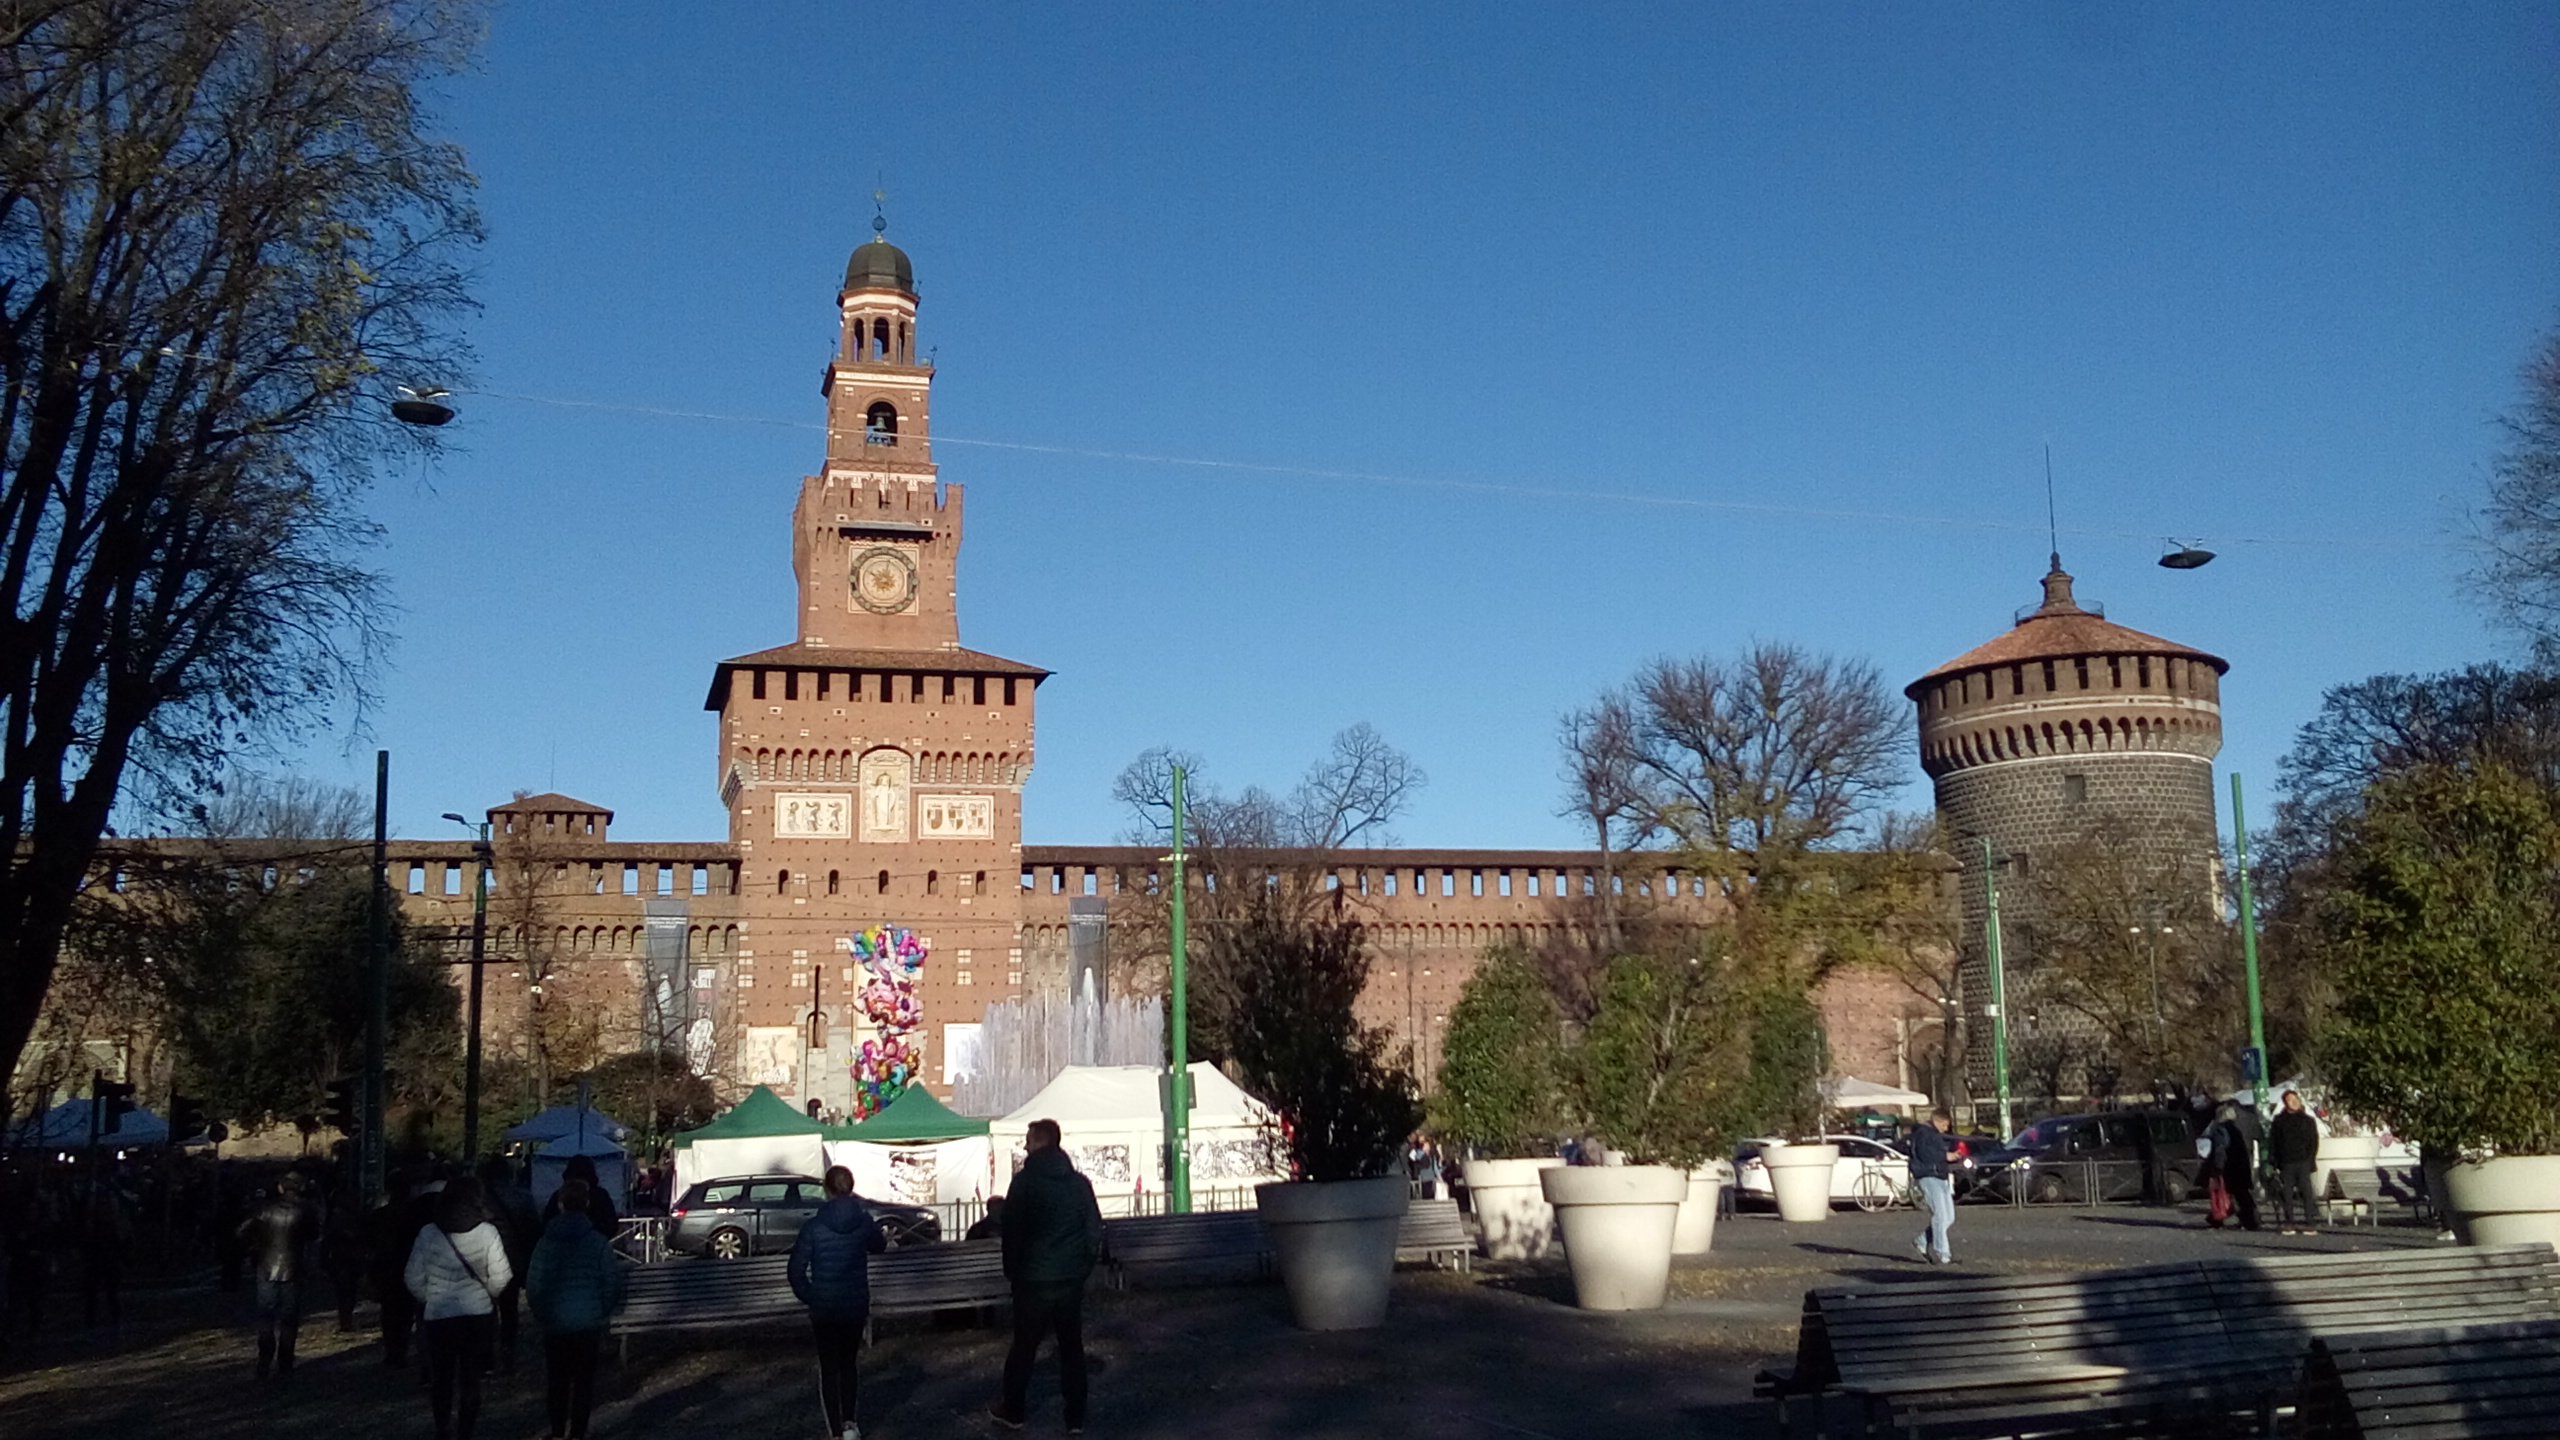
\includegraphics[width=\textwidth]{../../../References/Images/Dynamia/CastleOfDynamia/20181208_100357}
  \caption{Reference image for the Castle of Dynamia}
\end{figure}

\begin{figure}[H]
  \centering
  \includegraphics[width=6cm]{Images/Palettes/dynamiaCastle}
  \caption{Palette for the Castle of Dynamia}
\end{figure}

\begin{figure}[H]
  \centering
  \includegraphics[width=6cm]{Images/Palettes/dynamiaCastlePrison}
  \caption{Palette for the prison in the Castle of Dynamia}
\end{figure}

\begin{figure}[H]
  \centering
  \includegraphics[width=12cm]{Images/Maps/castleOfDynamiaFull}
  \caption{General map of the Castle of Dynamia}
\end{figure}

\begin{figure}[H]
  \centering
  \includegraphics[width=\textwidth]{Images/Maps/castleOfDynamia}
  \caption{Detailed map of the Castle of Dynamia}
\end{figure}

\begin{figure}[H]
  \centering
  \includegraphics[width=\textwidth]{Images/Maps/castleOfDynamiaFloorsPreview}
  \caption{Floors preview of the Castle of Dynamia}
\end{figure}

For more reference images: \url{http://wastelandsteam.altervista.org/dynamia/castle-of-dynamia/}\\
Password: \textit{gld18}

\subsection{Docking point}
\begin{figure}[H]
  \centering
  \includegraphics[width=\textwidth]{Images/Maps/dynamia_dockingPoint}
  \caption{Docking point position}
\end{figure}
  
In this area we may find wooden poles placed in the water, decorated with flowers, where gondoliers and fishers tie their little boats and gondolas, and  stone stairs that lead to small platforms on the canals.

In the center of the area there is a small street and a fountain which has in its middle a statue representing Mizar, surrounded by flowers. Mizar keeps her right arm up holding her scepter that spills water.

Behind the docking point the player can see the gigantic city walls that defend Dynamia from enemy attacks.

\begin{figure}[H]
  \centering
  \includegraphics[width=\textwidth]{Images/Landmarks/dockingPoint}
  \caption{References image for the docking point}
\end{figure}
For more reference images: \url{http://wastelandsteam.altervista.org/dynamia/docking-point/}\\
Password: \textit{gld18}
